\documentclass[a4paper,12pt]{article}
\usepackage{amssymb, amsmath} % needed for math
\usepackage{lmodern}
\usepackage[utf8]{inputenc}   % this is needed for umlauts
\usepackage[USenglish]{babel} % this is needed for umlauts
\usepackage[T1]{fontenc}      % this is needed for correct output of umlauts in pdf
\usepackage[margin=2.5cm]{geometry} %layout
\usepackage{color}
\usepackage{framed}
\usepackage{enumerate}  % for advanced numbering of lists
\usepackage{csquotes}   % for enquote
\usepackage{graphicx} % support the \includegraphics command and options
\usepackage{parskip} % no indent paragraph
\usepackage{microtype}
\usepackage{setspace} \onehalfspacing
\usepackage{hyperref}
\graphicspath{{img/}}


\title{DesCartes Builder specification}
\author{Eduardo de Conto}

\usepackage{microtype}

\begin{document}
\maketitle


\section{Introduction}

Rene is a framework and methodology for the integration of Hybrid AI tools and
components. At a high-level, we imagine the Builder to be a set of building
blocks (Lego pieces) for hybrid AI, alongside with a framework to connect these
building blocks together, validate them and execute them.

% CITE
Briefly, Hybrid AI is a type of artificial intelligence (AI) where
traditional AI models and physics or symbolic models are combined. The objective
here is, as suggested by Paco \& others, to adjust for the "ignorance" of our
models or the aspects that are not considered in the modeling.

With the DesCartes Builder, we aim to:
\begin{itemize}
  \item Integrate: merge and combine the hybrid AI tools for different type of
  physics (electricity, fluid dynamics, mechanics) and applications domains
  (energy, transportation, drone).
  \item Validate: ensure that tools and models work well together and can be
  applied to the final targeted application.
  \item Facilitate: make the development of hybrid AI models and applications
  easier.
\end{itemize}

\section{Features}
Here are some of the features we're considering and that can be meaningful to
implement here.
\begin{itemize}
  \item Definition of a pipeline building blocks
  \item Pipeline consistency checking
  \item Visual interface to define the pipeline
  \item Building blocks and libraries containing key models and packages for hybrid AI
  \item Import and export of existing models
  \item Experiment tracking
  \item Execution and export of models
\end{itemize}

\subsection{Building blocks}

We define a set of Objects and Operators that are manipulated by the Pipeline.

Objects can be either Data or Function:
\begin{itemize}
  \item \textbf{Data} corresponds to the numerical values to process, the physics measurements
  we're interested in.
  \item \textbf{Function} corresponds to the trained regression models (for
  traditional AI), the physics model, etc. It's anything that, when given data,
  will produce some transformed data.
\end{itemize}

Operators can either be Process, Code or Train. See Fig.~\ref{fig:blocks}.
\begin{figure}
  \centering
  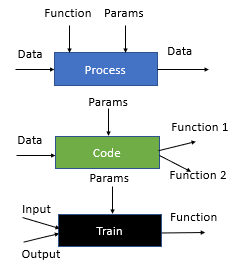
\includegraphics[width=0.3\textwidth]{building-blocks.png}
  \caption{\label{fig:blocks} Building blocks}
\end{figure}

\begin{itemize}
  \item \textbf{Code} Given one input Data stream $I$ and Parameters $P$,
  produce one or two Functions. The first function, $f_1$, encodes the data, and
  the second function, $f_2$, decodes the data. By encoding/decoding, we refer
  to the transform and inverse-transform operations of dimensionality reduction,
  such as PCA, POD, PGD.
$$
    I^* = f_1(I); I \approx f_2(I^*); \\
    I \in R^{n}\times R^{feat}; I^* \in R^{m}\times R^{feat}; m<<n
$$
  \item \textbf{Train} Given two Data stream, input $I$ and output $O$, produce one
  Function $f$. This Operator represents the supervised learning process. We expect
  that $f$ such that $O \approx f(I)$.
  \item \textbf{Process} Given some original Data, produce a transformed Data by
applying a Function. The Function is generated by the Code and Train nodes
above and, hence, doesn't need to be explicitly written.
\end{itemize}

\subsection{Consistency checking}
The goal of this consistency checking is to ensure that the pipeline is
consistent before executing. This is expected to save time from erroneous
executions.

\textbf{Process} ensures that:
\begin{itemize}
  \item the first input is the Function to be called
  \item other inputs are data and parameters
  \item the Function is compatible with the provided data: same number of inputs, etc.
  Will check that the Function is tagged with the same type of Data.
\end{itemize}

\textbf{Code} ensures that, given data with type $T_1$, we'll have
$F_1: T_1 \rightarrow T_2$ and $F_2: T_2 \rightarrow T_1$. That is, $F_1$ will accept
$T_1$ and produce a new type $T_2$. $F_2$ will accept $T_2$ and produce $T_1$.

\textbf{Train} Given two data streams (Input with type $T_I$ and Output with type
$T_O$) train will return a function $F: T_I \rightarrow T_O$.

\section{Implementation}

At this point, we're looking to leverage \textbf{Kedro} to implement the
Builder. Kedro provide a framework based on a dataflow model. In dataflow model, the computation is
define a set of nodes with data flowing between operations. The nodes define a
graph that can be execution. Kedro defines already for us:
\begin{itemize}
  \item the nodes
  \item the pipeline (as a combination of nodes)
  \item an infra-structure to run the pipeline
  \item management of the datasets and parameters of the pipeline
\end{itemize}

The concept behind Rene is similar to tools such as Ansys Twin Builder and
Modelica.

\section{Acronyms}
\begin{itemize}
  \item PCA: Principal Component Analysis
  \item POD: Proper Orthogonal Decomposition
  \item PGD: Proper Generalized Decomposition (extension of POD)
\end{itemize}


\end{document}
